\documentclass[12pt]{article}

\usepackage{graphicx,amsmath,amssymb,amsfonts}
\usepackage[margin=1in]{geometry}
\usepackage{hyperref}
\usepackage{natbib}
\usepackage{color}

\graphicspath{{../correlation_analysis/figures/}}

\begin{document}


\title{Predicting evolutionary site variability from structure in viral proteins: buriedness, flexibility, and design}
\author{Amir Shahmoradi, $^{1,2}$ %\footnote{$^{*}$ Authors with equal contributions.}
            Daria K. Sydykova,$^{2}$ Stephanie J. Spielman,$^{2}$ \\
            Eleisha L. Jackson,$^{2}$ Eric T. Dawson,$^{2}$ Austin G. Meyer,$^{2}$ Claus O. Wilke$^{2}$}

\date{\small $^1$ Department of Physics, The University of Texas at Austin, TX, 78712 \\
                 $^2$ Institute for Cellular and Molecular Biology, The University of Texas at Austin, TX, 78712 \\ }

\maketitle

\begin{abstract}
Several recent works have shown that site-specific evolutionary variation in proteins can be predicted from protein structure. Most prominently, sites that are buried and/or have many contacts with other sites in a structure evolve more slowly than surface sites with few contacts. Here, we present a comprehensive study of numerous different structural properties that may constrain sequence variation, including measures of buriedness (relative solvent accessibility, contact number), measures of structural fluctuations (B factors, root-mean-square fluctuations, variation in dihedral angles), and variability in designed structures. Structural fluctuation measures were obtained from molecular dynamics simulations performed on 9 non-homologous viral protein structures, and from variation in homologous variants of these proteins where available. Variability in designed structures was obtained from flexible-backbone design via Rosetta. We found that most of the structural properties correlate with site variation in the majority of structures, though the correlations are generally weak (correlation coefficients of 0.1 to 0.4). We further found that measures of buriedness tend to be better predictors of evolutionary variation than measures of structural fluctuations. Variability in designed structures was a weaker predictor of evolutionary variability than both measures of buriedness and measures of fluctuations. We conclude that simple measures of buriedness are better predictors of evolutionary variation than more complicated predictors obtained from dynamic simulations, ensembles of homologous structures, or computational protein design.
\end{abstract}


\section*{Introduction}

Identification of the driving factors in protein evolution has been on of the important objectives in molecular biology and protein research \citep{rocha_quest_2006,MarshTeichmann2014}. It is already well-established and understood that highly conserved amino acid sites in the protein sequences often fall in hotspot regions responsible for the protein's biophysical function or happen to be pivotal in maintaining the protein's native conformation \citep{li_proteinprotein_2004, keskin_hot_2005}. Aside from biophysical constraints, several structural determinants of protein dynamics and flexibility have been recently proposed to impose site-specific evolutionary pressure on the protein sequence. Examples include residue-level solvent exposure \citep{Ramseyetal2011,Scherreretal2012,MeyerWilke2013, other_authors}, local protein density \citep{liao_protein_2005, zhou_contact_2008, FranzosaXia2009, yeh_site-specific_2014}, and measures of residue-level flexibility of the protein backbone \citep{liu_sequence_2012, nevin_gerek_structural_2013}.

Among correlating variables, the Relative Solvent Accessibility (hereafter RSA) has gained special attention for its ability in predicting the general patterns of residue-level sequence variability and evolution in globular proteins. This variable is defined as a residue's site-specific Accessible Surface Area (ASA) to solvent molecules, normalized by the theoretically or experimentally determined maximum accessible area for the same residue \citep{Rose1985,Tienetal2013}. RSA was first introduced in the context of hydrophobicity scales derived by computational means from protein crystal structures \citep{Chothia1976, Rose1985, Miller1987} and its association with sequence variability may be explained in terms of the residue hydrophobicity which correlates strongly with RSA \citep{moelbert_correlation_2004}. The core of globular proteins is generally thought as a region of near-zero solvent accessibility that is mainly occupied by tightly-packed hydrophobic amino acid side chains. It can be therefore expected that any mutations of these hydrophobic residues in the protein core to hydrophilic or bulkier side chains may result in significant changes the native conformation of the protein \citep{munson_what_1996} which might in turn adversely affect the biophysical functioning of the protein and hence exert selection pressure against such mutations. In other words, the positive association of RSA with sequence variability is not a causal relation but merely a reflection of the effects of geometrical or chemical constraints on sequence variability.

Along with RSA, other measures of residue buriedness, such as residue contact number {\color{red}(e.g., Liao et al. 2005; Zhou et al. 2008; Franzosa \& Xia 2009; Yeh et al. 2012)} have been proposed and shown to correlate with sequence variability, or even argued to serve as better predictors than RSA.  Based on physical arguments and experimental evidence (xx what kind of arguments?), \citet{Halle2002} argued that the local residue packing density is a direct proxy measure of residue and site-specific backbone flexibility, in particular the Debye-Waller factors, commonly known as B factors. Therefore, given the strong observational evidence for the significant positive correlation of residue density and packing with sequence evolution \citep{Yehetal2014}, one may also expect to observe a positive trend between local flexibility and sequence variability. Indeed, several authors have argued for the potential role of protein dynamics on sequence variability \citep{liu_sequence_2012, nevin_gerek_structural_2013}.
	
Although multitude of structural variables have been shown or predicted to influence residue-level sequence variability, there is currently no consensus on which variable and to what extent has the dominant role in regulating sequence variability, independently of other structural determinants. So far, a comprehensive study of all potential structural determinants of protein sequence evolution has been missing in the literature, with the existing work mainly focusing on individual variables. In particular, measures of residue spatial fluctuations and protein dynamics have only received marginal attention and consideration as potential contributing factors to sequence evolution.

Proteins are intrinsically dynamic entities in vivo, far from their perceived rigidities in crystal structures and their dynamic behavior is expected to influence their sequence evolution \citep{MarshTeichmann2014}.  However, contrary to RSA and residue contact number, an accurate determination of the protein's dynamical behavior and residue fluctuations---solely based on the set of 3-dimensional atomic coordinates in crystal structures---remains a challenging task. B factors are generally considered as an attractive proxy to local flexibility, though the atomistic definition of B factor may not be appropriate for the study of side-chain flexibility and fluctuations. Experimental studies of protein dynamics in vivo has also proven extremely difficult if not impossible ({\color{red}Vendruscolo 2007}).

Alternatively, Molecular Dynamics (hereafter, MD) simulations provide an ideally suited method of studying protein dynamics and its potential role in driving sequence evolution.  Here in this work, we attempt to present a comprehensive study of several potential structural determinants of sequence variability from both protein crystallography and Molecular Dynamics perspectives. In addition to the factors already discussed in previous works, such as RSA and residue contact number, we also consider new dynamical measures of structural variability in the study, such as variance of the backbone and residue dihedral angles and residue spatial fluctuations from MD simulations and discuss their potential influence on sequence variability. The extent and breadth of such analysis however, limits diversity of the input data used in our work to highly evolving proteins that have multiple high-resolution homologous crystal structures in Protein Data Bank \citep{berman_protein_2008}. The availability of multiple structures is required for the calculation of site-specific spatial fluctuations and comparison of the results with the same variability measures based on MD simulations. In addition, the selected proteins should also have ample sequence data to ensure good statistic for sequence alignment and the calculation of sequence variability and evolutionary rates.
	
In the following sections, first we briefly present the methodology employed for data selection, sequence alignments, data analysis and the procedure for obtaining the relevant structural variables from Molecular Dynamics simulations and homologous structures, followed by the results and a discussion of the potential contributors to sequence variability or evolution. We show that measures of residue buriedness such as RSA and contact number outperform site-specific measures of residue fluctuations and discuss the potential underlying biases and reasons contributing to this observation.

\section*{Materials and Methods}

\section*{Sequence data, alignments, and evolutionary rates}

All viral sequences except influenza and HIV sequences were retrieved from \url{http://hfv.lanl.gov/components/sequence/HCV/search/searchi.html}.
The sequences were truncated to the desired genomic region but not in any other way restricted. Influenza sequences were downloaded from \url{http://www.fludb.org/brc/home.spg?decorator=influenza}. We only considered human influenza A, H1N1, excluding H1N1 sequences from the 2009 Swine Flu outbreak. We only used sequences from after 1998 but did not place geographic restrictions.
%HIV-1 sequences were retrieved from \url{http://www.hiv.lanl.gov/components/sequence/HIV/search/search.html}.
%Sequences were truncated to the desired genomic region, but no other restrictions were imposed.

For all viral sequences, we removed any sequence that was not in reading frame, any sequence which was shorter than 80\% of the longest sequence for a given viral protein (so as to remove all partial sequences), and any sequence containing any ambiguous characters. Alignments were constructed using amino-acid sequences with MAFFT \citep{Katohetal2002,Katohetal2005}, specifying the ``--auto" flag to select the optimal algorithm for the given data set, and then back-translated to a codon alignment using the original nucleotide sequence data.

To assess site-specific sequence variability in amino-acid alignments, we calculated the Shannon entropy ($H_i$) at each alignment column $i$:
\begin{equation}
        H_i = - \sum_jP_{ij}\ln P_{ij}.
\end{equation}
Here, $P_{ij}$ is relative frequency of amino acid $j$ at position $i$ in the alignment.

For each alignment, we also calculated evolutionary rates, as described \citep{SpielmanWilke2013}. In brief, we generated a phylogeny for each codon alignment in RAxML \citep{RaxMLHPC} using the GTRGAMMA model. Using the codon alignment and phylogeny, we inferred evolutionary rates with a Random Effects Likelihood (REL) model, using the HyPhy software \citep{KosakovskyPondetal2005}. The REL model was a variant of the GY94 evolutionary model \citep{GoldmanYang1994} with five $omega$ rate categories as free parameters. We employed an Empirical Bayes approach \citep{Yang2000} to infer $dN/dS$ values for each position in the alignment. The amino-acid sequence of the seed protein structures were then mapped to the corresponding alignments for subsequent analyses.
%Additionally, using the phylogenies inferred with RAxML, we calculated a phylogenetic weight for each sequence using BranchManager \citep{Stone2007}.

\subsection*{Molecular Dynamics Simulations}

Molecular dynamics (MD) simulations were carried out using the GPU implementation of the {\it Amber12} simulation package (cite xx) with the most recent release of Amber fixed-charge force field (ff12SB; c.f., AmberTools13 Manual).
		
Prior to MD production runs, all PDB structures were first energy minimized using the steepest descent method for 1000 steps, followed by conjugate gradient for another 1000 steps. Then, the structures were constantly heated from 0K to 300K for 0.1ns, followed by 0.1ns constant pressure simulations with positional harmonic restraints on all atoms to avoid instabilities during the equilibration process. The systems were then equilibrated for another 5ns without positional restraints, each followed by 15ns of production simulations for subsequent post-processing and analyses. All equilibration and production simulations were run using the SHAKE algorithm (cite xx), {\color{blue}by which all bonds involving hydrogen are constrained to avoid instabilities for a choice of 2fs time step in simulations.} Langevin dynamics were used for temperature control (cite for Langevin dynamics xx).

\subsection*{Measures of buriedness and of structural flexibility}

As measures of residue buriedness, we calculated Relative Solvent Accessibility (RSA), contact number (CN), and weighted contact number (WCN). To calculate RSA, we first calculated the Accessible Surface Area (ASA) for each residue in each protein, using the DSSP software \citep{KabschSander1983}. We then normalized ASA values by the theoretical maximum ASA of each residue \citep{Tienetal2013} to obtain RSA. We calculated CN for each residue as the total number of C$\alpha$ atoms surrounding the  C$\alpha$ atom of the focal residue within a spherical neighborhood of a predefined radius $r_0$. Following \citet{Yehetal2014}, we used $r_0=13\AA$. We calculated WCN as the total number of surrounding C$\alpha$ atoms for each focal residue, weighted by the inverse square separation between the C$\alpha$ atoms of the focal residue and the contacting residue, respectively \citep{Shihetal2012}.

In most analyses, we actually used the inverse of CN and/or WCN, $\text{iCN}=1/\text{CN}$ and $\text{iWCN}=1/\text{WCN}$. Note that for Spearman correlations, which we use throughout here, replacing a variable by its inverse changes the sign of the correlation coefficient but not the magnitude.

As measures of structural variability, we considered RMSF, variability in backbone and side-chain dihedral angles, and B factors. {\color{blue}Based on MD trajectories, we calculated RMSF for the backbone C$\alpha$ atoms of all protein structures with respect to the corresponding coordinates of the PDB crystal structures listed in Table \ref{tab:pdb_names}. In addition, the same RMSF measurements were carried out based on the structural alignments for four protein families that had adequate number of homologous structures in Protein Data Bank}

To assess variability in backbone and side-chain dihedral angles, we calculated Var($\phi$), Var($\psi$), and Var($chi_1$). {\color{red}The variance of a dihedral angle is defined as \dots.} Since the $\chi_1$ angle is undefined for Ala and Gly we excluded all sides with these residues in analyses involving $\chi_1$.

B factors were extracted from the crystal structures listed in Table~\ref{tab:pdb_names}. We only considered the B factors of the C$\alpha$ atom of each residue.

\subsection*{Protein crystal structures}
	
A total of $8$ viral proteins were selected for analysis, as tabulated in Table \ref{tab:pdb_names}.

\subsection*{Sequence Entropy from Designed Proteins}

Design entropy was calculated as described \citep{Jacksonetal2013}. In brief, proteins were designed using RosettaDesign (Version 39284) \citep{LeaverFayetal2011} using a flexible backbone approach. This was done for all PDB structures in Table \ref{tab:pdb_names} as initial template structures. For each template, we created a backbone ensemble using the Backrub method \citep{Smith2008}. The temperature parameter in Backrub was set to 0.6, allowing for an intermediate amount of flexibility.  For each of the 9 template structures we designed 100 proteins.

\subsection*{Availability of data and methods}

All details of simulations, input$/$output files and scripts for subsequent analyses are available to view or download at \url{https://github.com/clauswilke/structural\_prediction\_of\_ER}.

\section*{Results}

\subsection*{Data set and structural variables considered}

Our goal in this work is to determine which structural properties best predict amino-acid variability at individual sites in proteins. To this end, we selected 9 viral proteins for which we had both high-quality crystal structures and abundant sequences to assess evolutionary variability (Table~\ref{tab:pdb_names}). We quantified evolutionary variability in two ways, by calculating entropies for each alignment column (sequence entropy) and by calculating the evolutionary-rate ratio $\omega=dN/dS$ (see Methods for details). Throughout this paper, we primarily report results obtained for sequence entropy. Results for $\omega$ are largely comparable, with some specific caveats detailed below.

As predictors of evolutionary variability, we considered two broad classes of structural properties, residue buriedness and residue flexibility. Measures of buriedness quantify the extent to which a residue is protected from solvent. A commonly used measure of buriedness is solvent-accessible surface area (ASA) or its normalized variant relative solvent accessibility (RSA). Here we considered RSA, since it can be compared among residues of different sizes. We also considered contact number (CN) and weighted contact number (WCN). Both of these quantities assess the number of other residues a focal residue contacts. CN simply counts the number of contacts within a sphere of a given radius around the $\alpha$-carbon of the focal residue. WCN weights contacts by the distance between the two residues. Note that residue buriedness decreases as RSA increases, but it increases with increasing CN or WCN. To avoid this difference in directionality, in most analyses we replaced CN and WCN with their inverse, iCN=1/CN and iWCN=1/WCN. Because nearly all analyses we carried out were non-parametric and only depended on the rank order of the variables, this substitution only changed the sign of correlations but not the magnitude.

Measures of flexibility assess the extent to which a residue fluctuates in space as a protein undergoes thermodynamic fluctuations in solution. There are different ways to quantify these fluctuations. First, we can measure the root mean-square deviation of the C$\alpha$ atom over time. This quantity is commonly called RMSF. Second, we can consider B factors, which measure the spatial localization of individual atoms in a protein crystal. Third, we can measure the variability in side-chain or backbone dihedral angles, such as Var($\chi_1$), Var($\phi$), or Var($\psi$). Here, we considered all these measures of structural variability.

To calculate measures of flexibility, we generated molecular-dynamics (MD) trajectories for all crystal structures in Table~\ref{tab:pdb_names}. In all cases, we equilibrated the structure and then simulated 15ns of chemical time (see Methods). We recorded snapshots of the simulated structure every 10ps. From these snapshots, for each residue we calculated RMSF as well as the variability in dihedral and side-chain angles. We also calculated time-averaged values of the three measures of buriedness RSA, CN, and WCN. We refer to these time-averaged values as MD RSA, MD CN, and MD WCN, respectively.


\subsection*{Structural buriedness vs.\ structural flexibility as predictors of evolutionary variation}

We first compared a subset of variables among the measures of buriedness and measures of fluctuations in their explanatory power for sequence variation. Figure~\ref{fig:cor_entropy_all} shows the Spearman correlation between sequence entropy and each of the quantities RSA, iWCN, Var$(\chi_1)$, RMSF, and B factor, for each protein. Significant correlations ($P<0.05$) are shown with filled symbols, and non-significant correlations are shown with empty symbols ($P\geq0.05$).
In this figure, several patterns emerge. First, all correlations are generally positive and significant. The main exception is the RNA binding domain of Marburg virus, PDB ID 4GHA, which mostly shows no correlation but shows a negative correlation between sequence entropy and the variability in the $\chi_1$ angle. Second, correlations are generally weak. No correlation coefficient exceeds 0.4. Third, on average the correlation strength decreases as we move from left to right in the figure. The two measures of buriedness, RSA and iWCN, show the strongest correlations. Their correlations are on average $\rho=0.26$ and $\rho=0.22$, respectively. The three fluctuation measures Var($\chi_1$), RMSF, and B factor exhibit weaker correlations, on average $\rho=0.17$, $\rho=0.10$, and $\rho=0.13$, respectively.

We next analyzed structural fluctuations more carefully, by comparing the correlations of entropy with six different measures of local structural flexibility.  We considered variations in the backbone and side-chain dihedral angles ($\phi$, $\psi$, and $\chi_1$), B factors, RMSF obtained from MD simulations, and RMSF obtained from crystal structures. For the latter quantity, we aligned homologous structures with distinct sequences, obtained from the PDB (see Methods for details). The correlation strengths of these quantities with entropy are shown in Figure~\ref{fig:cor_entropy_SF}. We found that the variation in backbone dihedral angles Var($\phi$) and Var($\psi$) explained the least variation in sequence entropy, while the variation in the side-chain dihedral angle Var($\chi_1$) explained, on average, more variation in sequence entropy than any other measure of structural flexibility. B factors and the two measures of RMSF explained on average approximately the same amount of variation in entropy, even though the results for individual proteins were discordant (see also next sub-section).

\subsection*{MD time-averages vs.\ crystal-structure snapshots}

For most analyses discussed so far, except analyses involving B factors or crystal RMSF, we averaged structural quantities over MD trajectories comprising 15ns of chemical time. This is not conventional practice for quantities such as RSA or contact numbers. Instead, most authors simply obtain these quantities from individual crystal structures. We therefore asked whether MD averages differed in any meaningful way from estimates obtained from crystal structures, and whether estimates from MD and from crystal structures different in their predictive power for sequence variability.

We found that RSA, CN, and WCN from crystal structures were highly correlated with their averages over MD trajectories, for all protein structures we examined (Spearman correlation coefficients of $>0.9$ in all cases {\color{red}Can we put these into a table?}). Further, when we correlated these quantities with sequence entropy, we found that the correlation coefficients we obtained for each protein were virtually identical (Figure~\ref{fig:cor_cr_md}A-C). Thus, in terms of predicting evolutionary variation, RSA and contact numbers obtained from the static structures performed as well as their dynamic equivalents averaged over short time scales.

However, the same was not true when we considered backbone flexibility as measured by root mean fluctuations (RMSF). RMSF cannot be obtained from a single crystal structure, but we can calculate it from an alignment of multiple crystal structures were available. When we compared RMSF from MD to RMSF from crystal structures, we found that they were generally quite different. In particular, the strength of the correlation between site entropy and RMSF from MD was independent of the strength of the correlation between site entropy and RMSF from crystal structures (Figure~\ref{fig:cor_cr_md}D). In fact, for the structure for which RMSF from MD had the highest explanatory power for site entropy {\color{red}(Which structure is this?)}, the RMSF from crystal structures had the least explanatory power for site entropy (Figure~\ref{fig:cor_cr_md}D). The reverse was also true. {\color{red}(Which is the structure for which RMSF from crystal structure works best?)}

To further investigate the relationship between backbone fluctuations and sequence variability, we also compared the RMSF correlations to the correlations between sequence entropy and B factors. Again, we found that these correlations were generally different from the ones found for either the MD RMSF or the crystal structure RMSF (Figure \ref{fig:cor_entropy_bfca_rmsf}). Thus, B factors, MD RMSF, and crystal RMSF, though all measures of backbone fluctuations, contained distinct information about sequence variability in our data set.

\subsection*{Sequence entropy vs.\ evolutionary-rate ratio $\omega$}

In the previous subsections, we have used sequence entropy as a measure of amino-acid variability at individual sites. While sequence entropy is a simple and straightforward measure of site variability, it has two potential drawbacks: First, entropy doesn't correct for the phylogenetic relationship of sequences in the alignment, and hence it can be biased if some parts of the phylogeny are more densely sampled than others. Second, entropy does not take into account the actual substitution process. As a result, a single substitution near the root of the tree can result in a comparable entropy to a sequence of substitutions toggling back and forth between two amino acids.

To consider an alternative quantity of sequence variability that doesn't suffer from either of these drawbacks, we calculated the evolutionary-rate ratio $\omega=dN/dS$ for all proteins at all sites, and repeated all analyses with $\omega$ instead of entropy. We found that all results generally carried over, but the correlations tended to be somewhat weaker. Figure~\ref{fig:cor_entropy_omega} plots, for each protein, the correlation between $\omega$ and the various structural quantities versus the correlation between entropy and the same structural quantities. We see that all data points generally fall below the $x=y$ line, and are shifted downwards by approximately 0.1. Thus, correlations of structural quantities with $\omega$ are, on average, approximately 0.1 smaller than correlations of the same quantities with entropy.

Besides the measures of buriedness and measures of structural flexibility discussed in the previous subsections, we present in  Figure~\ref{fig:cor_entropy_omega} one additional structural quantity, \emph{design entropy}. Design entropy is obtained by using computational protein design to generate artificial alignments of designed sequences, and then measuring sequence entropy in these artificial alignments. We had previously shown that design entropy captures some of the variation observed in natural alignments \citep{Jacksonetal2013}. Here we found that design entropy performed about as well as the measures of structural flexibility but worse than the measures of buriedness.

\subsection*{Multi-variate analysis of structural predictors}

The various structural quantities we have considered are by no means independent of each other. Measures of buriedness co-vary with each other, as do measures of structural flexibility. Further, the latter co-vary with the former, as does design entropy. To determine the extent to which the various quantities contain independent information about sequence variability, and to assess whether combining multiple structural quantities yields improved predictive power, we carried out a joint multivariate analysis including most of the structural quantities considered in this work. The approach we used is a principal component (PC) regression, which has previously been used successfully to disentangle genomic predictors of whole-protein evolutionary rates \citep{Drummondetal2006,Bloometal2006}. In this analysis, we first carry out a principal component analysis of the predictor variables (i.e., the structural quantities such as RSA and RMSF), and we then regress the response (sequence entropy or $\omega$) against the individual components.

Because we wanted to analyze all proteins in our data set individually but in such a way that results were comparable from one protein to the next, we pooled all structural quantities for a single PC analysis and then regressed entropy and $\omega$ against each PC separately for each protein. The results of this analysis are shown in Figure~\ref{fig:cor_entropy_PC_screen}.
{\color{blue} Need to finish this. A few more sentences of what we actually found. }

\section*{Discussion}

{\color{blue}Put a summary paragraph here.}


{\color{blue}One paragraph about the \citep{Yehetal2014} paper and RSA vs. CN.}

We have found that correlations between sequence entropy and structural quantities were consistently higher than correlations between the evolutionary-rate ratio $\omega$ and structural quantities. This difference likely reflects the distinct physical processes that entropy and $\omega$ measure. Entropy is a measure of the amino-acid diversity allowed at a given site. In effect, it reflects how many different amino acids are allowed. By contrast, $\omega$ measures how rapidly amino-acid changes occur at a given site. While entropy and $\omega$ are generally correlated, a site can have high entropy and comparatively low $\omega$ and vice versa. In particular, if mutations rapidly toggle back and forth between two different amino acids at a site, then that site will have high $\omega$ and low entropy. By contrast, if a site diversified into a number of different alleles deep in the phylogeny but did not experience much further evolution at later times, then that site will have comparatively high entropy but low $\omega$. Since structural quantities such as measures of buriedness reflect the biophysical constraints imposed on sites, it makes sense that they would be better predictors of the allowed amino-acid diversity at a site than the speed of substitution at that site. By contrast, biological processes such as immune escape would likely be better predictors of substitution rates than amino-acid diversity.

The correlation strengths we have observed here between evolutionary variation and structural quantities were consistently lower than those observed in prior work \citep{Jacksonetal2013,Yehetal2014}. We believe that this result was due to our choice of analyzing viral proteins instead of the cellular proteins or enzymes used in prior works. First, while viral sequences are abundant, their alignments may not be as diverged as alignments that can be obtained for sequences from cellular organisms. For example, our influenza sequences spanned only approximately one decade. Despite the high mutation rates observed in RNA viruses, the evolutionary variation that can accumulate over this kind of time span is limited. And the lower the evolutionary divergence, the harder it becomes to resolve differences between more and less conserved sites in a protein. Second, many viral proteins experience a substantial amount of selection pressure to evade host immune responses. The resulting positive selection on viral sequences may mask evolutionary constraints imposed by structure. For example, influenza hemagglutinin displays positive selection throughout the entire sequence, and both at buried and at exposed sites \citep{MeyerWilke2013,Meyeretal2013,Suzuki,Bush}.

{\color{blue}One paragraph about design and backbone flexibility}


\bibliographystyle{MBE}  % natbib.sty
\bibliography{Structural_prediction_of_ER.bib}%%%refs.bib

\newpage

\section*{Tables}

\begin{table}[htbp]
\caption{\textbf{PDB structures considered in this study.}\label{tab:pdb_names}}
\smallskip

\centerline{
\begin{tabular}{c c c c c} % c}
                        \hline
    Viral Protein   &  PDB ID  & Chain    & Sequence  & Number of   \\ 
    &    &       & Length    & Sequences   \\\hline                                                           
  Hemagglutinin Precursor         & 1RD8           & AB        & 503                & 1039        \\
  Dengue Protease Helicase        & 2JLY           & A         & 451                & 2362        \\
  West Nile Protease              & 2FP7           & B         & 147                & 237         \\
  Japanese Encephalitis Helicase  & 2Z83           & A         & 426                & 145         \\
  Hepatitis C Protease            & 3GOL           & A         & 557                & 1021        \\
  %Hepatitis C Protease            & 3GSZ           & A         & 558                & 1021        \\
  %Hepatitis C Protease            & 3I5K           & A         & 566                & 1021        \\
  Rift Valley Fever Nucleoprotein & 3LYF           & A         & 244                & 95          \\
  Crimean Congo Nucleocapsid      & 4AQF           & B         & 474                & 69          \\
  Marburg RNA Binding Domain      & 4GHA           & A         & 122                & 42          \\
  Influenza Nucleoprotein         & 4IRY           & A         & 404                & 943         \\
  \hline
\end{tabular}
}
\end{table}

\begin{table}[htbp]
\caption{\textbf{Availability of homologous crystal structures.} \label{tab:homologs}}
\smallskip

\centerline{
\begin{tabular}{c c c c c c}
                        \hline
  Viral Protein & BLAST hits$^\text{a}$ & \multicolumn{4}{c}{Unique sequences} \\ 
    \cline{3-6}\noalign{\smallskip}
                &            & all  & $\geq2$\%$^\text{b}$  &  \textbf{$\mathbf{\geq}$5\%}$^\text{b}$  & $\geq10$\%$^\text{b}$ \\\hline
  Hemagglutinin Precursor         & 57 & 12 & 7 & \textbf{5} & 4\\
  Dengue Protease Helicase        & 31 & 11 & 7 & \textbf{7} & 6\\
  West Nile Protease              & 16 & 15 & 6 & \textbf{6} & 2\\
  Japanese Encephalitis Helicase  & 31 & 12 & 7 & \textbf{7} & 6\\
  Hepatitis C Protease            & 277 & 32 & 10 & \textbf{5} & 4 \\
  Rift Valley Fever Nucleoprotein & 95  & 9 & 5 & \textbf{5} & 5\\
  Crimean Congo Nucleocapsid      & 7 & 4 & 3 & \textbf{1} & 1\\
  Marburg RNA Binding Domain      & 40 & 6 & 3 & \textbf{3} & 3\\
  Influenza Nucleoprotein         & 69 & 19 & 4 & \textbf{4} & 2\\
  \hline
\end{tabular}
}
$^\text{a}$ Excluding all hits with $<35$\% sequence identity and $<90$\% alignment length\\
$^\text{b}$ Unique sequences at indicated minimum pairwise sequence divergence
\end{table}

\cleardoublepage

\section*{Figures}


\begin{figure}[tbh]
\begin{center}
    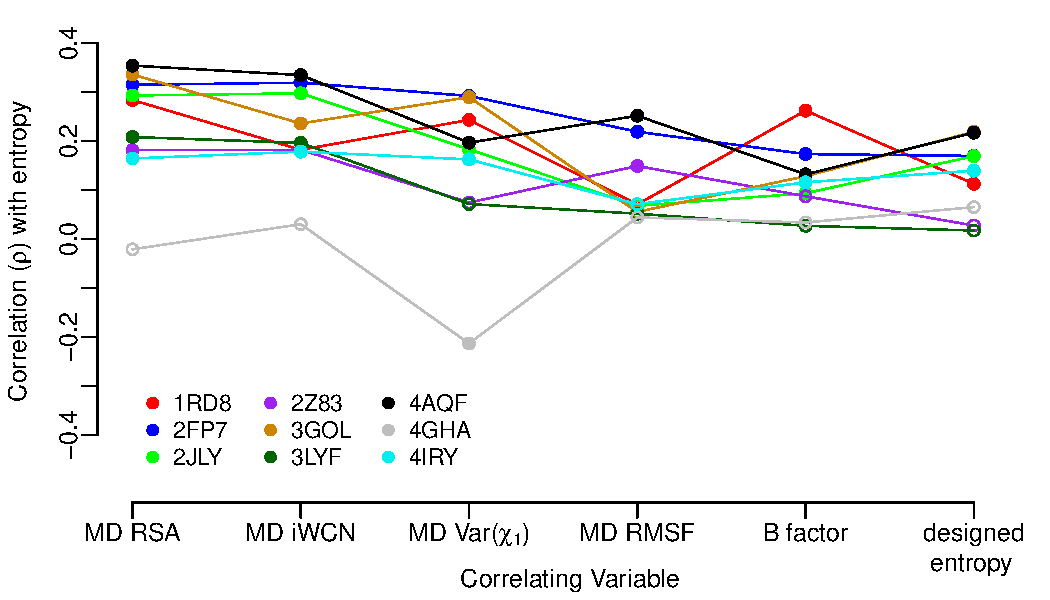
\includegraphics[width=5in]{cor_entropy_all.pdf}
\end{center}
\caption{\textbf{Spearman correlation of sequence entropy with measures of buriedness and of structural variability.} Each symbol represents one correlation coefficient for one protein structure. Significant correlations ($P<0.05$) are shown as filled symbols, and insignificant correlations ($P\leq0.05$) are shown as open symbols. The quantities RSA, iWCN, Var($\chi_1$), and RMSF were obtained as time-averages over 15ns of MD simulations. B factors were obtained from crystal structures. Compared to the measures of structural variability, the buriedness measures consistently show stronger correlations with sequence entropy.}
\label{fig:cor_entropy_all}
\end{figure}


\begin{figure}[tbh]
\begin{center}
    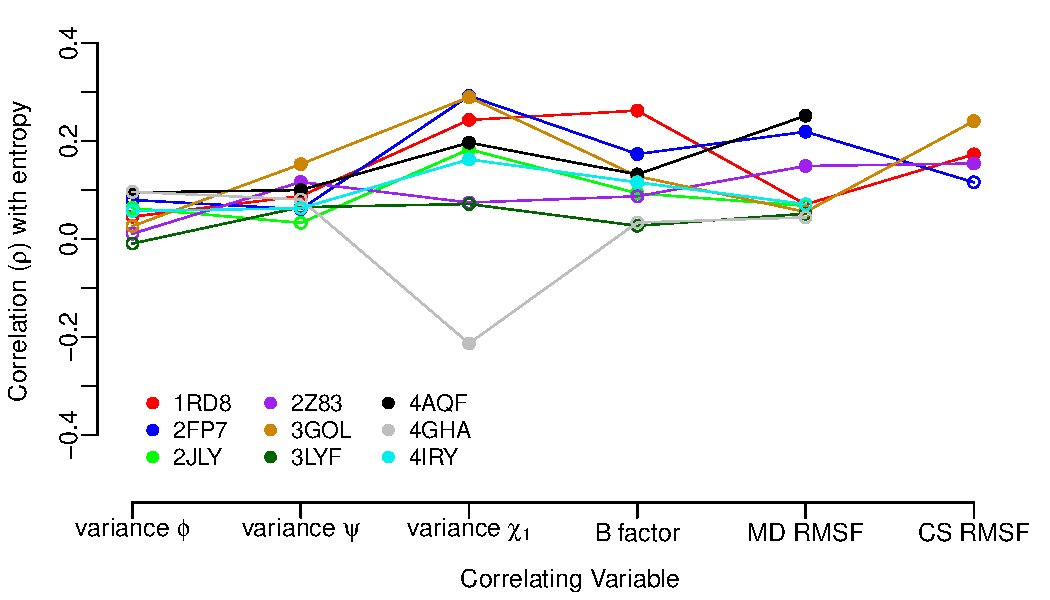
\includegraphics[width=5in]{cor_entropy_SF.pdf}
\end{center}
\caption{\textbf{Spearman correlation of sequence entropy with measures of structural variability.} Each symbol represents one correlation coefficient for one protein structure. Significant correlations ($P<0.05$) are shown as filled symbols, and insignificant correlations ($P\leq0.05$) are shown as open symbols. The quantities Var($\psi$), Var($\phi$), Var($\chi_1$), and MD RMSF were obtained as time-averages over 15ns of MD simulations. B factors were obtained from crystal structures. CS RMSF values were obtained from alignments of homologous crystal structures. Almost all structural measures of variability correlate weakly but significantly with sequence entropy.}
\label{fig:cor_entropy_SF}
\end{figure}

\begin{figure}[tbh]
\begin{center}
    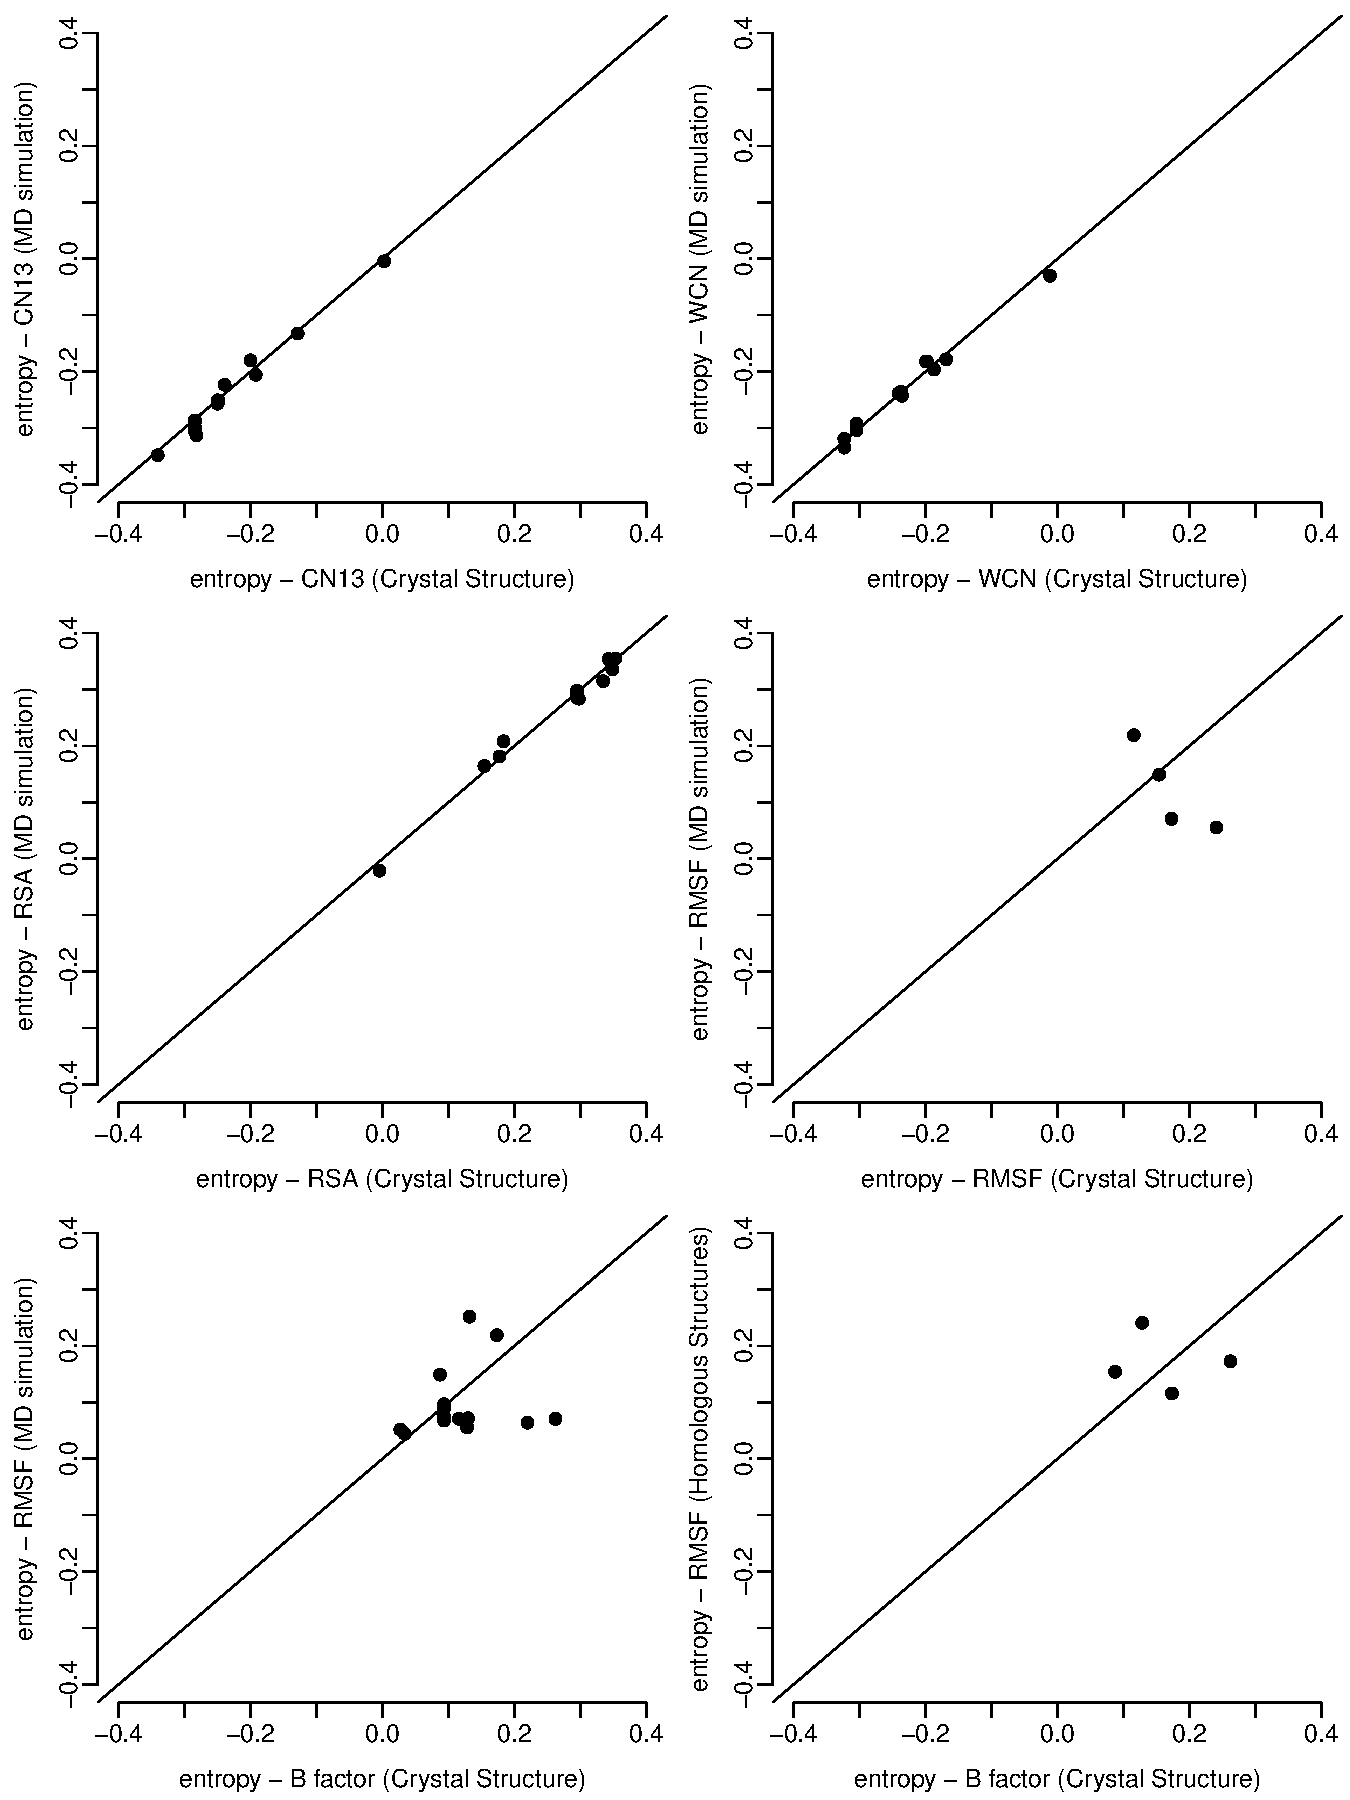
\includegraphics[width=6.5in]{cor_cr_md.pdf}
\end{center}
\caption{\textbf{Spearman correlations of sequence entropy with MD-derived and crystal-structure derived structural measures.}
The vertical axes in all plots represent the Spearman correlation of sequence entropy with one structural variable obtained from $15ns$ of Molecular Dynamics (MD) simulations. The horizontal axes represent the Spearman's rank correlation coefficient of sequence entropy with the same structural variable as in the vertical axes but measured from protein crystal structures. Each dot represents one correlation coefficient for one protein structure. The quantities iCN, iWCN, and RSA have nearly identical predictive power for sequence entropy regardless of whether they are derived from MD simulations or from crystal structures. By contrast, RMSF from MD simulations leads to very different correlations than RMSF from crystal structures does.
}
\label{fig:cor_cr_md}
\end{figure}

\begin{figure}[tbh]
\begin{center}
    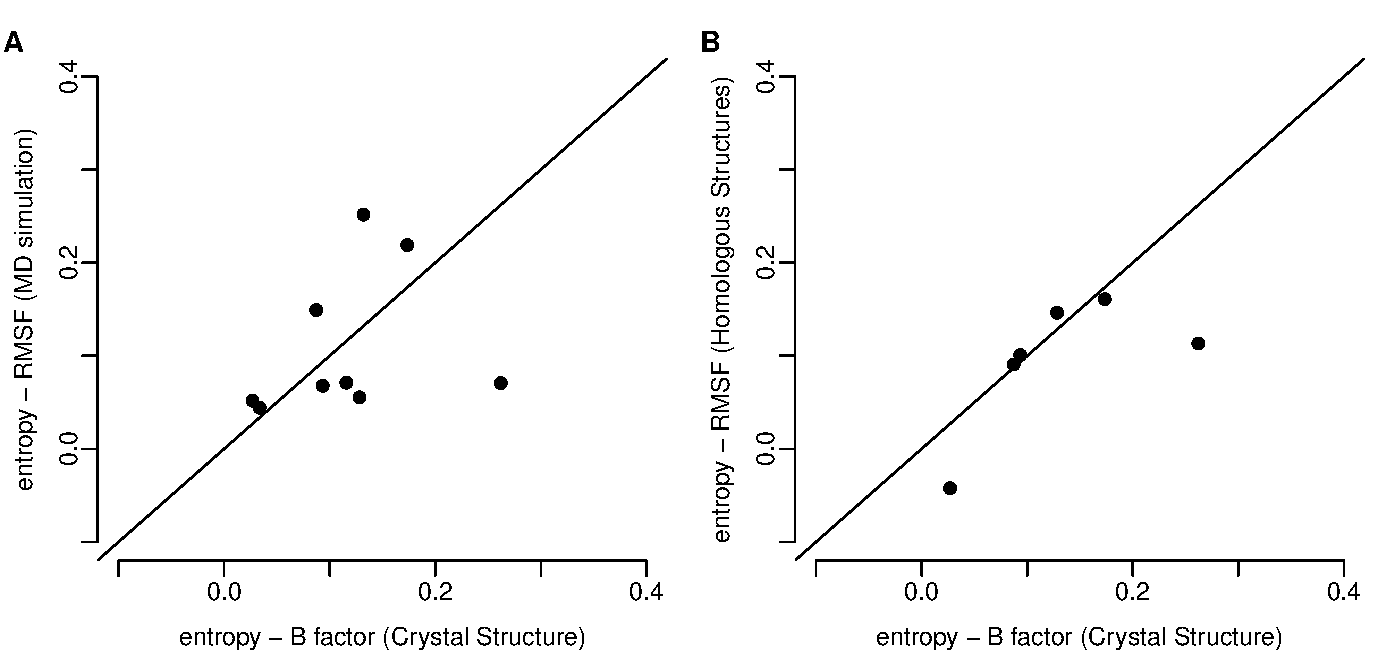
\includegraphics[width=6.5in]{cor_entropy_bfca_rmsf.pdf}
\end{center}
\caption{\textbf{Spearman correlations of sequence entropy with measures of structural variability.}
Vertical and horizonal axes represent Spearman correlations of the indicated quantities. Each dot represents one correlation coefficient for one protein structure. MD RMSF, crystal-structure RMSF, and B factors all have explain different amounts of variance in sequence entropy for different proteins.}
\label{fig:cor_entropy_bfca_rmsf}
\end{figure}

\begin{figure}[tbh]
\begin{center}
    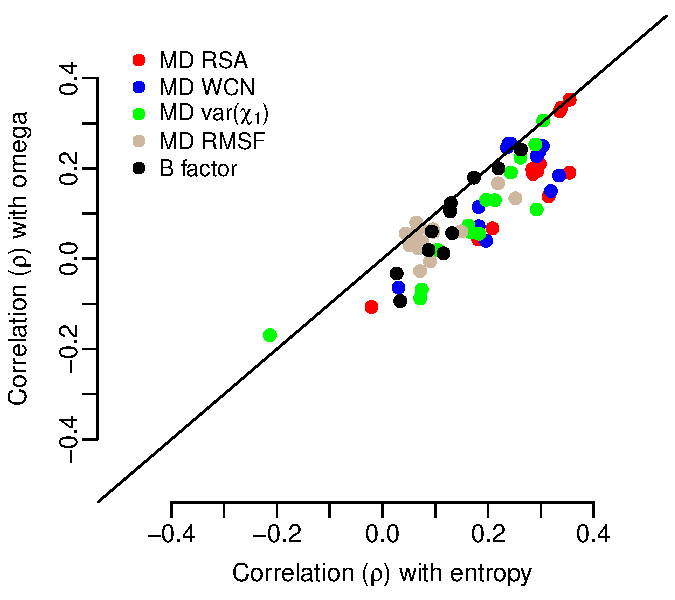
\includegraphics[width=4in]{cor_entropy_omega.pdf}
\end{center}
\caption{\textbf{Spearman correlations of structural quantities with sequence entropy and with the evolutionary rate ratio $\omega$.} All structural quantities generally predict as much as or more variation in sequence entropy than in $\omega$.}
\label{fig:cor_entropy_omega}
\end{figure}

\begin{figure}[tbh]
\begin{center}
       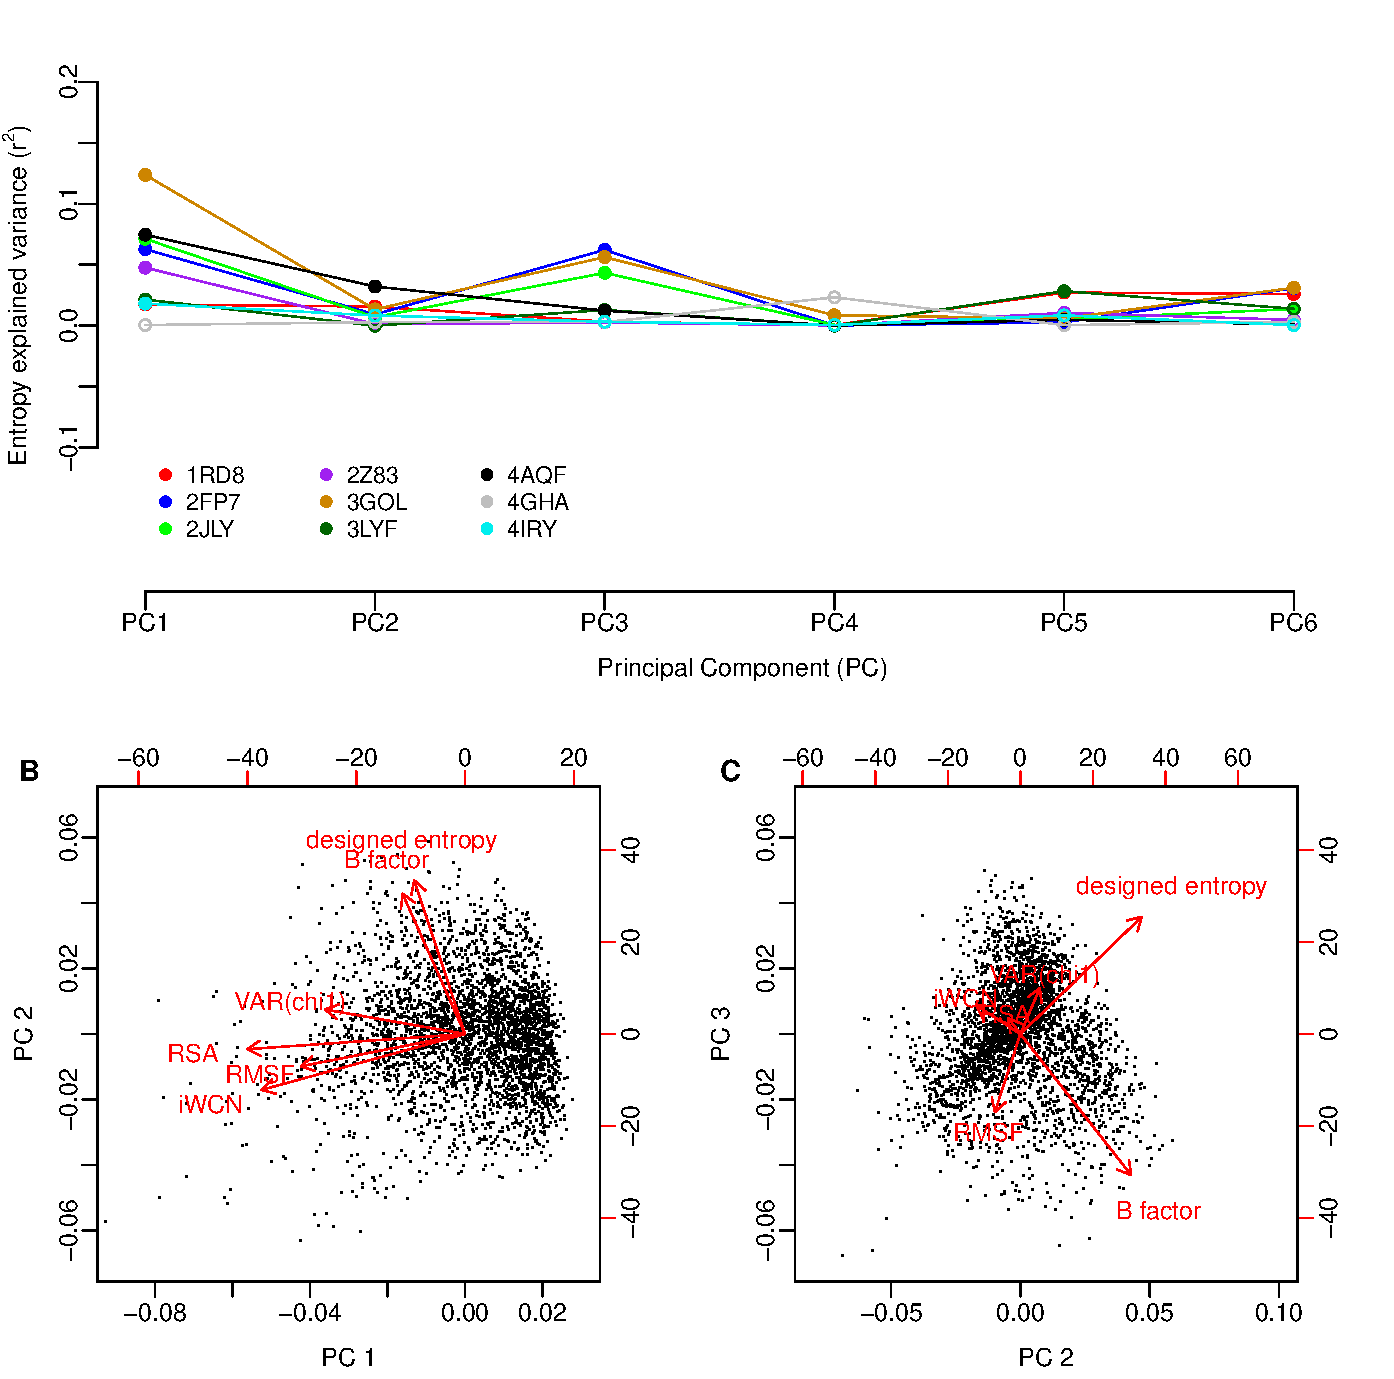
\includegraphics[width=6.5in]{cor_entropy_PC_screen.pdf}
\end{center}
\caption{\textbf{Principal Component (PC) Regression of sequence entropy given the structural variables.} {\bf (A)} Variance in entropy explained by each principal component. For most proteins, PC1 and PC3 show the strongest correlations with sequence entropy. Significant correlations ($P<0.05$) are shown as filled symbols, and insignificant correlations ($P\leq0.05$) are shown as open symbols. {\bf (B)} and {\bf (C)} Composition of the three leading components. Red arrows represent the loadings of each of the structural variables on the principal components; black dots represent the amino acid sites in the PC coordinate system. The variables RSA, iWCN, RMSF, and Var($\chi_1$) load strongly on PC1 and weakly on PC2, while B factor and design entropy load strongly on PC2 and weakly on PC1. Interestingly, B factor and design entropy also load strongly on PC3, but in opposite directions.}
\label{fig:cor_entropy_PC_screen}
\end{figure}

\end{document}
